\section{Event identification}
During production, runs were taken in batches of three, one each with \snTwelve,
\snFour, and the blank samples. Because the distance to each time-of-flight detector
was already measured, the time-of-flight for elastically-scattered neutrons could
be directly calculated and used to determine the delay from electronics and cabling.
The timestamp of each event was thus adjusted by a fixed amount
so that the first peak of the neutron spectrum aligned the expected
time-of-flight. Next, background $\gamma$-ray events were separated from relevant
neutron events by a pulse-shape discrimination analysis, shown in Fig. \ref{PHPSDPlot}.

\begin{figure}[tb]
    \centering
    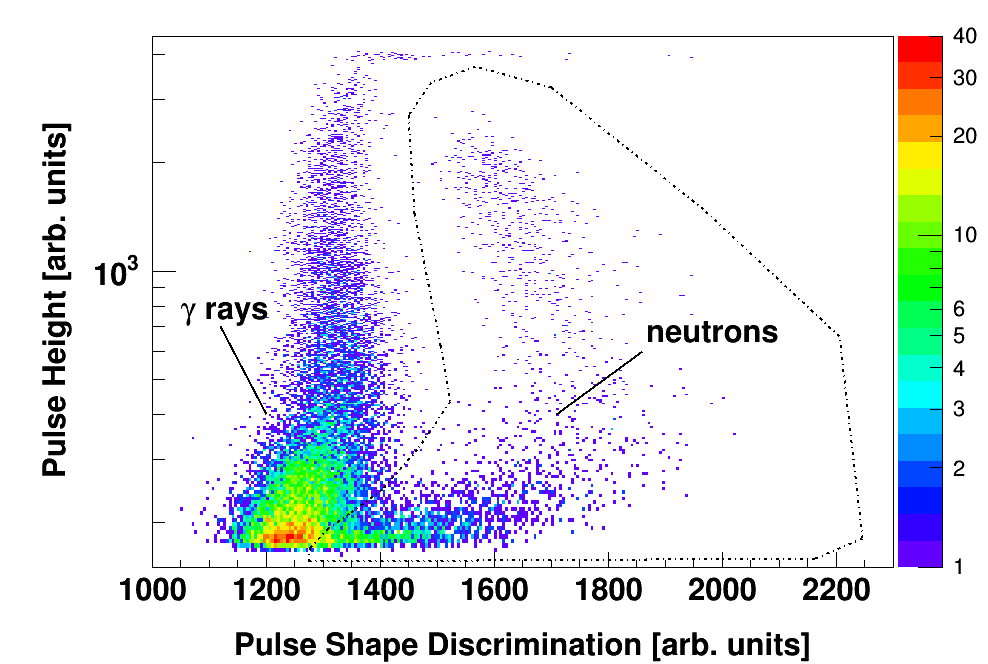
\includegraphics[width=0.9\textwidth]{figures/PHPSDPlot.png}
    \caption[Event pulse height (PH) vs. pulse-shape-discrimination (PSD) for
    a typical run]
    {
        Event pulse height (PH) vs. pulse-shape-discrimination (PSD) for
        a typical run. A gate (dashed line) isolates neutron events, which are
        used for subsequent analysis. At low pulse heights, the PSD output from the
        MPD-4 module is non-linear, making neutron-$\gamma$-ray separation more difficult
        (bottom-left of the figure).
    }
    \label{PHPSDPlot}
\end{figure}

%Neutron events surviving this PSD gating are shown for a few typical runs in Fig. 
%\ref{tiledRunData}. The first and second subfigures in the left column of the figure are from 
%the same detector and arm angle, but the first is from a blank-sample run and
%the second is from a \snFour\ sample-run. In each subfigure, the expected location
%of the time-of-flight for elastic scattering on \snFour\ is marked with a dark blue arrow,
%and the approximate FWTM time
%resolution of the detector is marked with blue dashed lines. The expected
%location of the time-of-flight peak for elastic scattering on atmospheric
%N$_{2}$ is marked with a green arrow. The additional counts in the 55-57 ns region in
%the second subfigure (compared to the first) are from elastic scattering on
%\snFour. Energy-dependent detector efficiencies for each detector were provided by TUNL
%and are shown above each histogram. For clarity, these efficiencies are plotted
%relative to the efficiency of at the elastically-scattered neutron energy.
%
%\begin{figure}[tb]
%    \centering
%    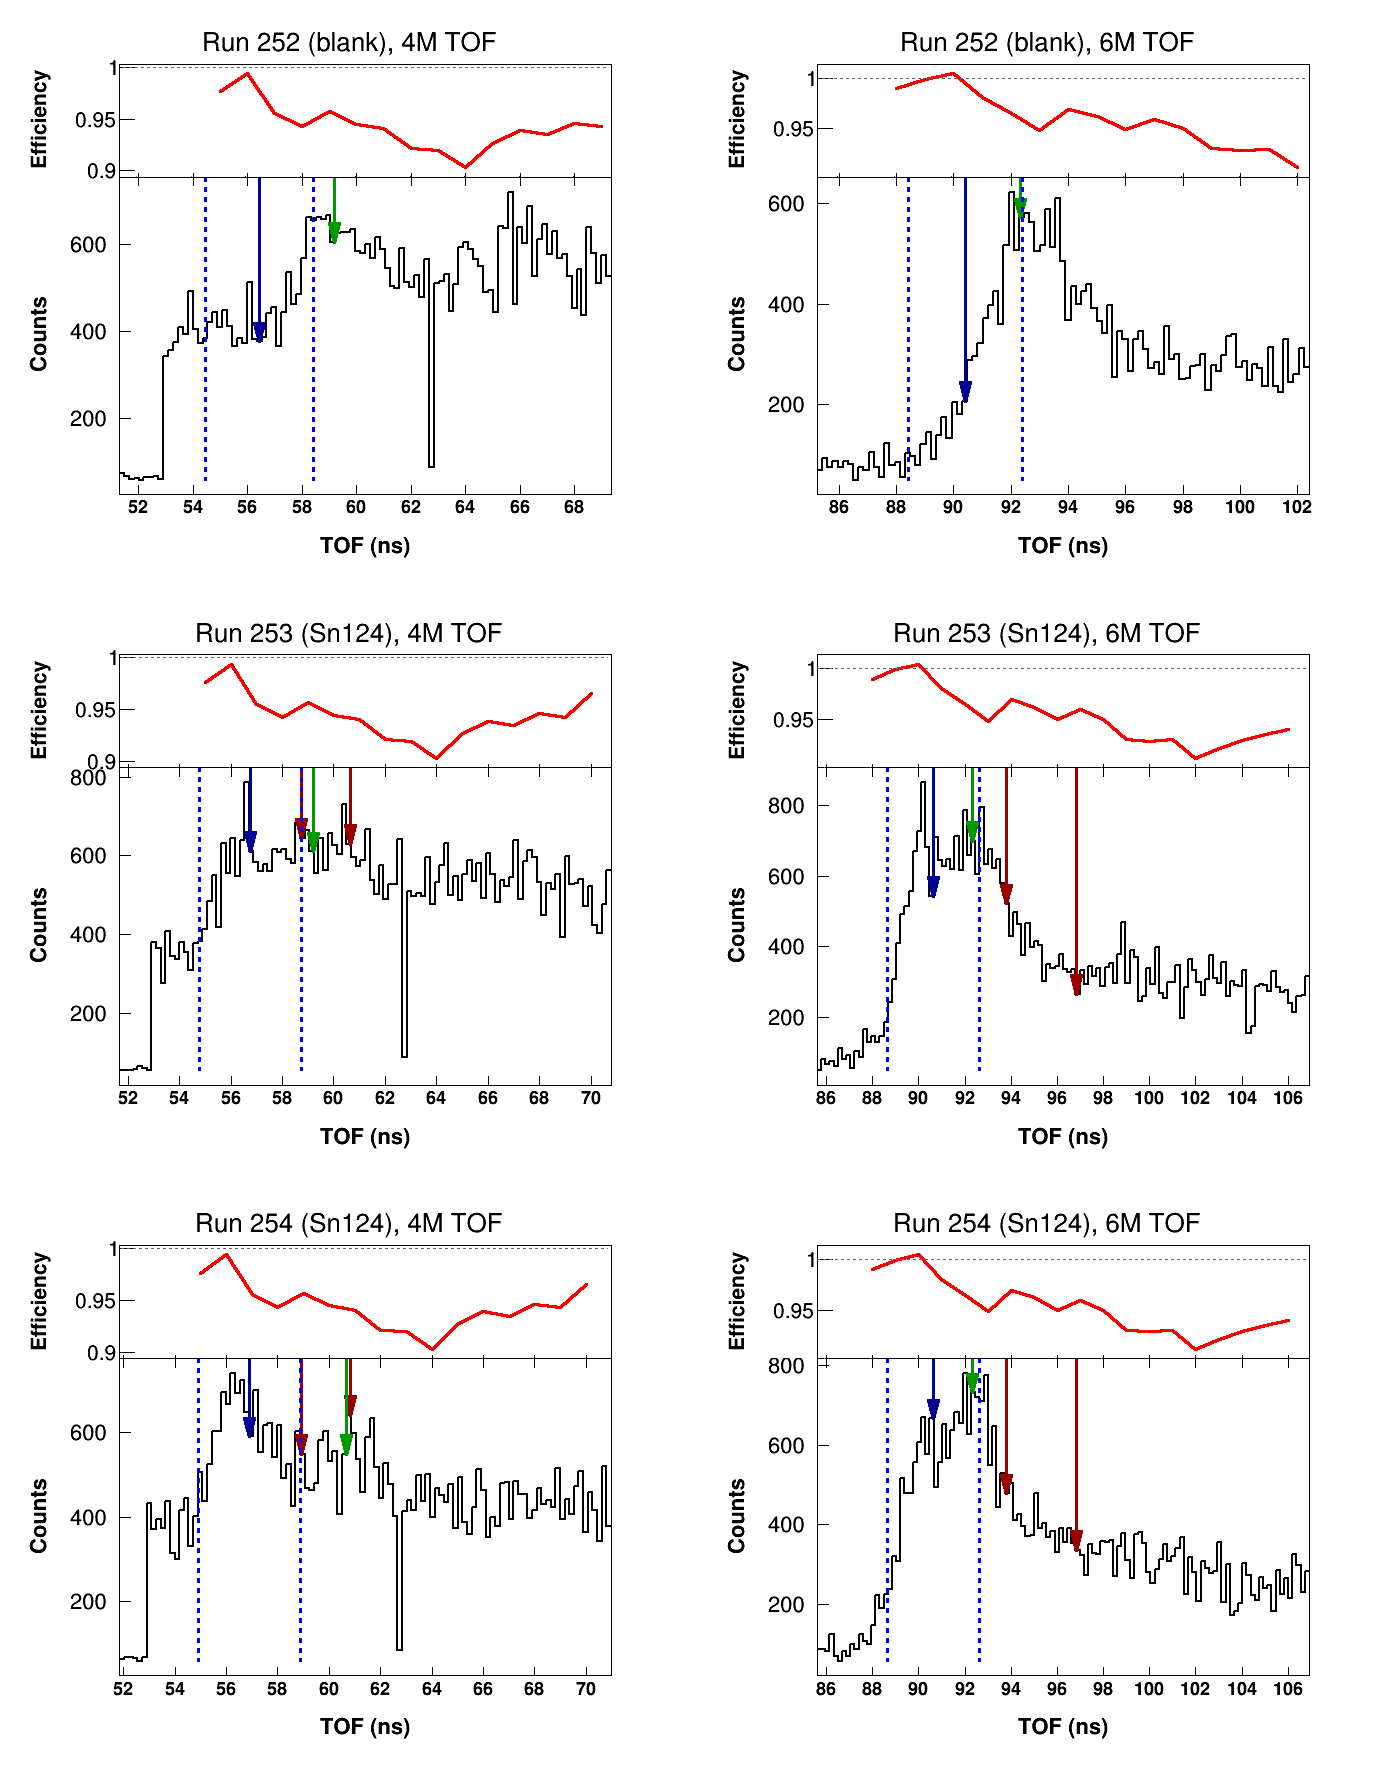
\includegraphics[height=0.6\textheight]{figures/tiledRunData.png}
%    \caption[Histograms from typical runs showing neutron elastic scattering peak]
%    {
%        Neutron-event histograms for three typical runs, one with the blank
%        sample and two with the \snTwelve\ sample.
%        In the first two rows, the expected locations of the \snTwelve\ elastic scattering peak 
%        (blue arrow)
%        and inelastic scattering peak from the first two excited states (red arrows) show an
%        increased number of counts compared to the last run (bottom row), which used the blank
%        sample. For reference, the expected location of the nitrogen elastic scattering
%        peak is shown with green arrow in all histograms.
%        The energy-dependent detector efficiency is plotted in the upper section of
%        each panel.
%    }
%    \label{tiledRunData}
%\end{figure}

After scaling histogram counts by detector efficiency, histograms were
normalized by the total neutron flux
(i.e., total counts in the CMON detector for that run) and summed by detector
angle. Then, blank-run histograms
were subtracted from the isotopic-run histograms to yield the neutron scattering
events from the isotopic samples. Figure \ref{tiledAngleData} provides example 
results. As in the previous figure, dark blue arrows mark the anticipated
time-of-flight of the elastic scattering peak, green arrows mark elastic
scattering from atmospheric nitrogen, and blue dashed lines mark the anticipated
full-width-tenth-maximum (FWTM) of the elastic scattering peak.
Inelastic scattering peaks from the first and
second excited states are marked with light blue
arrows. For the 4M detector and at forward angles for both detectors, the elastic and first 
inelastic scattering peaks are closer in time and cannot be cleanly resolved. Measurements in this
kinematic regime are the most challenging as the increased overlap between
these peaks increases the uncertainty of the number of counts in the elastic
peak. We fit the amplitudes of two Gaussian distributions to the elastic and
first-inelastic peaks while fixing
the width and centroid of each Gaussian according to our time-of-flight resolution and
the expected time-of-flight. The integral of the first Gaussian provides the
number of counts in the elastic peak.

\begin{figure}[ht]
    \centering
    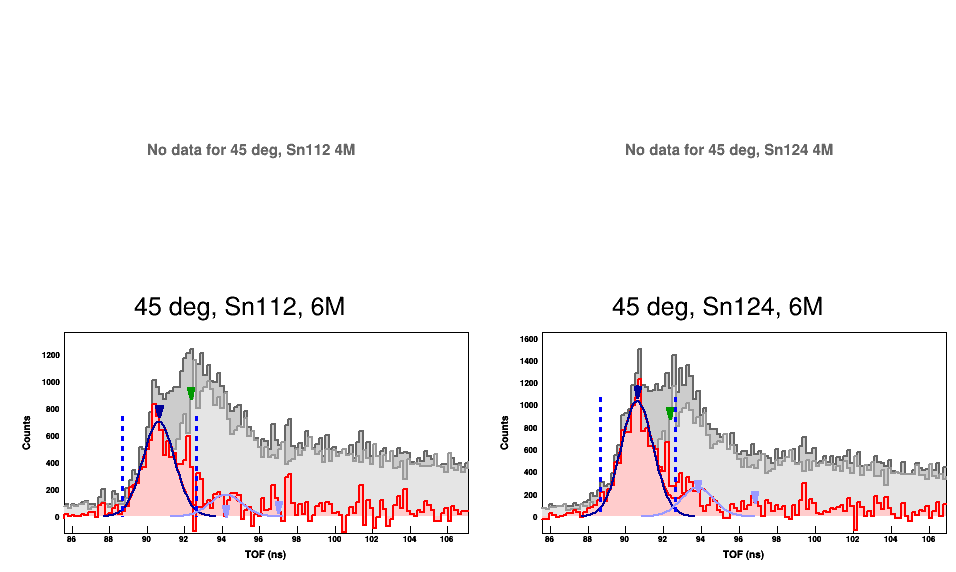
\includegraphics[width = 1.0\textwidth]{figures/tiledAngleData.png}
    \caption[Scaled event histograms showing neutron elastic scattering peak]
    {
        Scaled event histograms showing neutron elastic scattering and first
        inelastic scattering peaks from the 4M detector for a few representative angles. The
        histograms for isotopic-sample runs (dark gray),
        blank-sample runs (light gray), and the difference (in red) are shown.
        For each difference histogram, a double-Gaussian function
        was constructed with the centroid and width of each Gaussian fixed
        according to the expected time-of-flight for the elastic and first
        inelastic peaks and the detector resolution. The heights of each
        Gaussian were fitted to the difference histogram and the results of the
        fit are shown in dark blue (elastic peak) and light blue (first-inelastic peak).
    }
    \label{tiledAngleData}
\end{figure}

\section{Normalization}
To normalize the cross sections, a reference point is needed that connects the
neutron flux (as measured by the monitor detector) to a known cross section.
We took several reference runs using a graphite,
a polyethylene, and a blank sample at both the beginning and end of the experiment.
Figure \ref{ECSReferenceRuns} shows histograms for the 4M and 6M detectors for
one set of these runs, taken at 30\textdegree in the lab frame.
The same conventions from Fig.
\ref{tiledAngleData} are used, except that now the light blue arrows correspond to
the elastic and first-excited states of \cTwelve. The dark gray histogram (back
histogram layer) shows the elastic and first-excited states
of \cTwelve\ and also a broad peak from elastic scattering on H.
After scaling for the number
of moles in the graphite and polyethylene samples, stoichiometry, and neutron
flux, the graphite spectrum (light gray, middle histogram later) was subtracted from the polyethylene
spectrum, yielding neutron events only from elastic scattering on protons (area of
the red histogram between the blue dashed lines). As the cross section for
(n,p) scattering is extremely well-known, the number of counts in the
time-of-flight detectors in the reference run can be pegged to the absolute
differential cross section.
We used the Scattering Analysis Interactive Database (SAID) code \cite{SAIDCode}
to provide the (n,p) cross section at the energies and angles of the reference
runs, and using the reference cross section, the \snTwelveFour\
\el\ were normalized as:
\begin{equation} \label{ECSCalculation}
    \el(\theta) = \el_{ref}(\theta)
    \times \frac{X_{sample}}{X_{ref}} \times
    \frac{N_{sample}}{N_{ref}}
\end{equation}

\noindent
where $\el_{ref}(\theta)$ is the (n,p) cross section at lab angle $\theta$, $X_{sample}$
and $X_{ref}$ are number of counts in the flux-normalized elastic scattering peak for the sample
and the reference runs, respectively (see Figs. \ref{tiledAngleData} and
\ref{ECSReferenceRuns}), and $N_{sample}$ and $N_{ref}$ are the number of atoms in
the sample of interest and the number of hydrogen atoms in the polyethylene
sample, respectively.

\begin{figure}[tb]
    \centering
    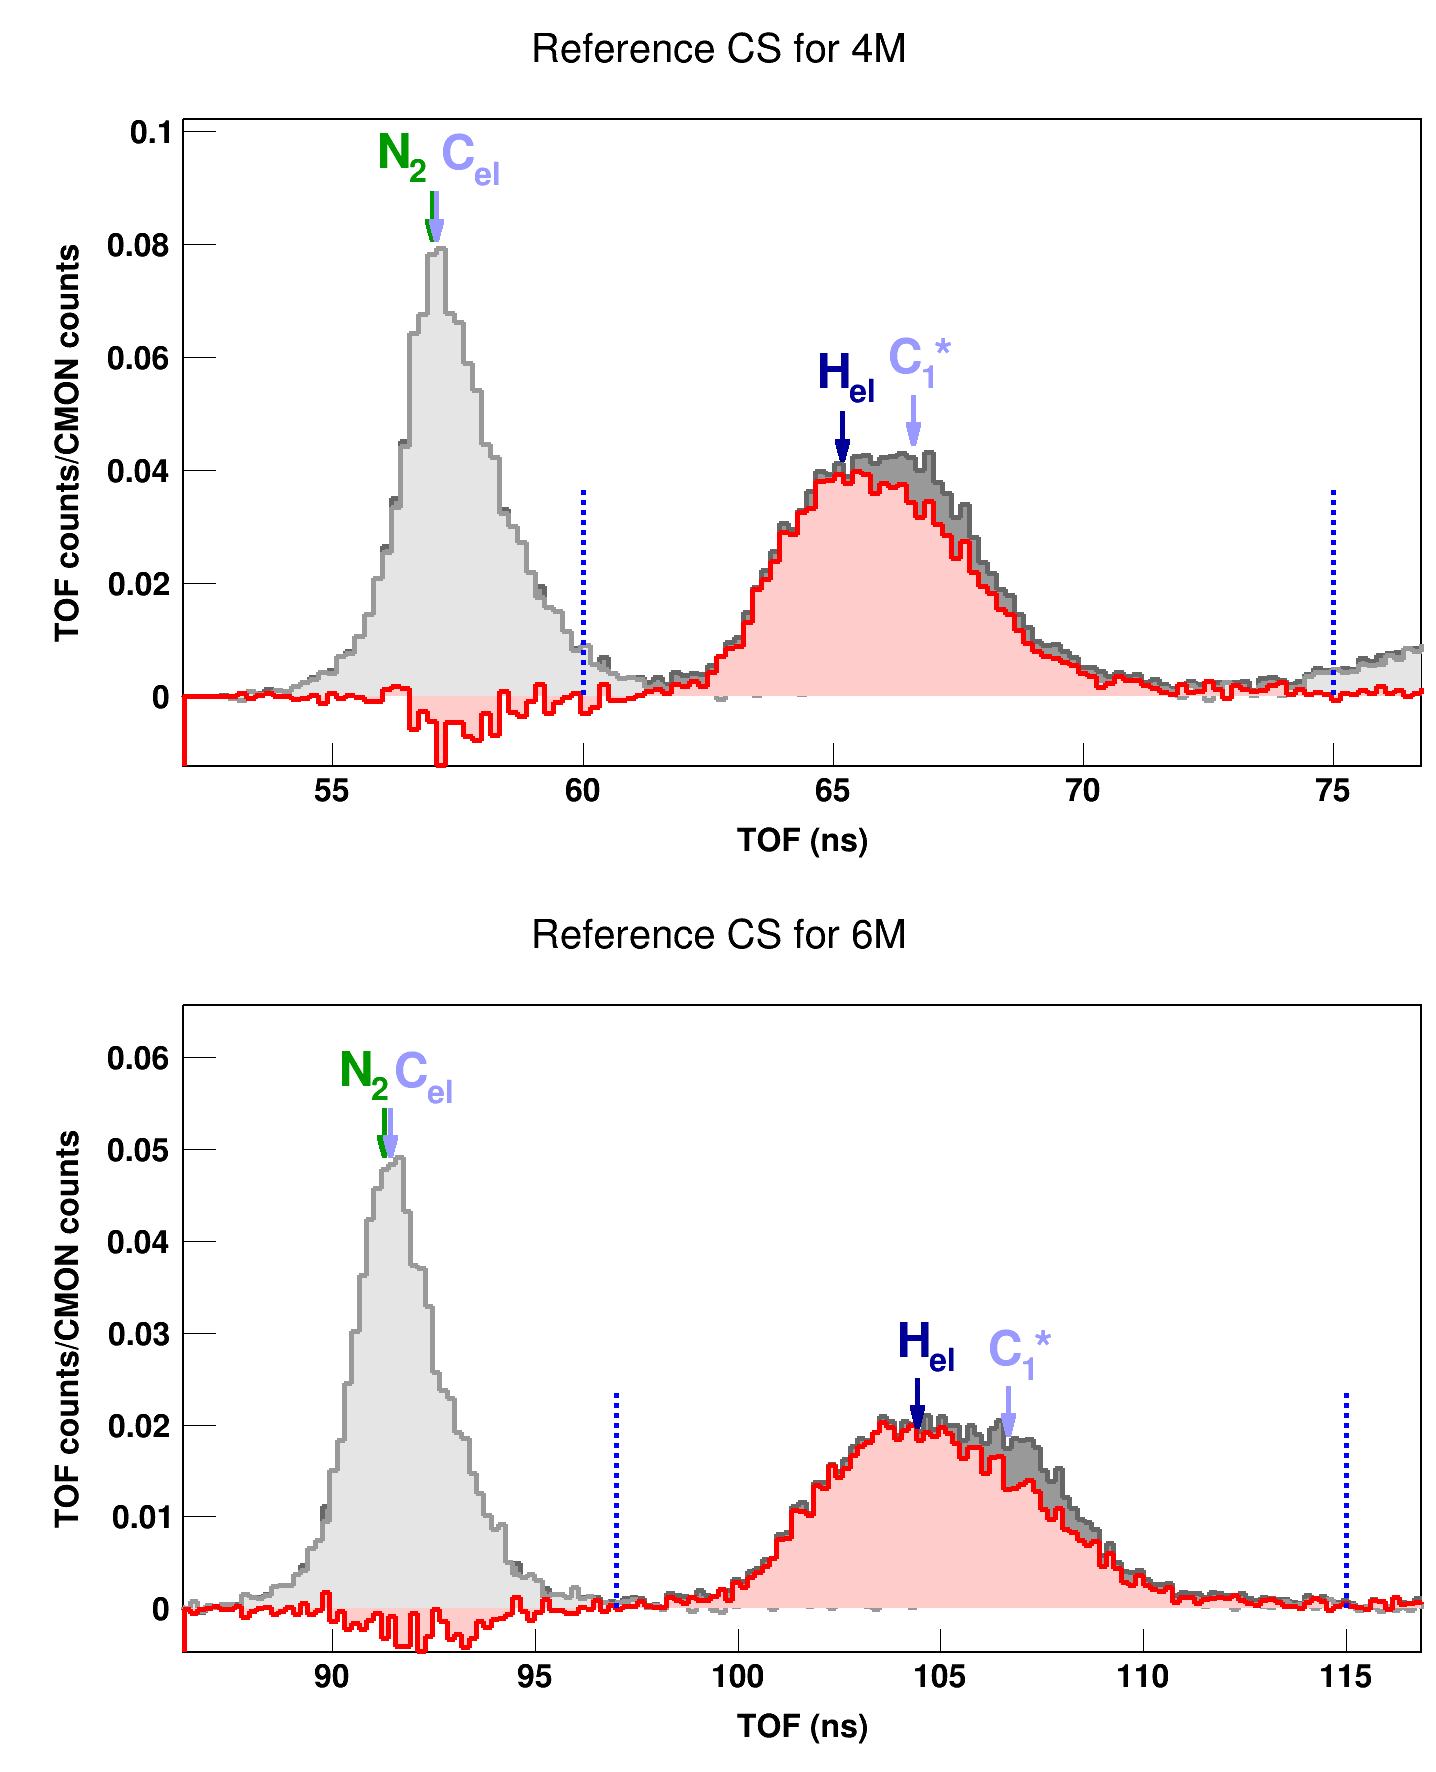
\includegraphics[height=0.7\textheight]{figures/ECSReferenceRuns.png}
    \caption[Reference runs of neutron scattering on C and (CH$_{2}$)$_{n}$]
    {
        Reference runs of neutron scattering on C and (CH$_{2}$)$_{n}$.
        The (CH$_{2}$)$_{n}$ run (back histogram, in dark gray) and C run
        (middle histogram, in light gray) are scaled by beam flux and number of
        atoms in each sample. Their difference (front histogram, in red) shows a
        broad peak corresponding to neutron-proton elastic scattering. The
        expected time-of-flight for neutrons elastically scattered from protons
        is shown by the blue arrow and aligns with the observed peak. Similarly,
        the light blue arrows 
        indicate the expected times-of-flight associated with neutron elastic and
        first-excited-state inelastic scattering on C.
        The green arrow indicates the expected time-of-flight of 
        neutrons elastically scattered on atmospheric N$_{2}$.
    }
    \label{ECSReferenceRuns}
\end{figure}

\section{Finite-Size Corrections}
In an idealized differential cross section measurement, the sample and neutron
detectors can be treated as point objects. In reality, the neutron beam,
samples, and detectors occupy a finite size (as illustrated in \ref{GussFiniteSizeDiagram},
leading to so-called finite-size effects that distort the measured cross sections.
\begin{figure}[tb]
    \centering
        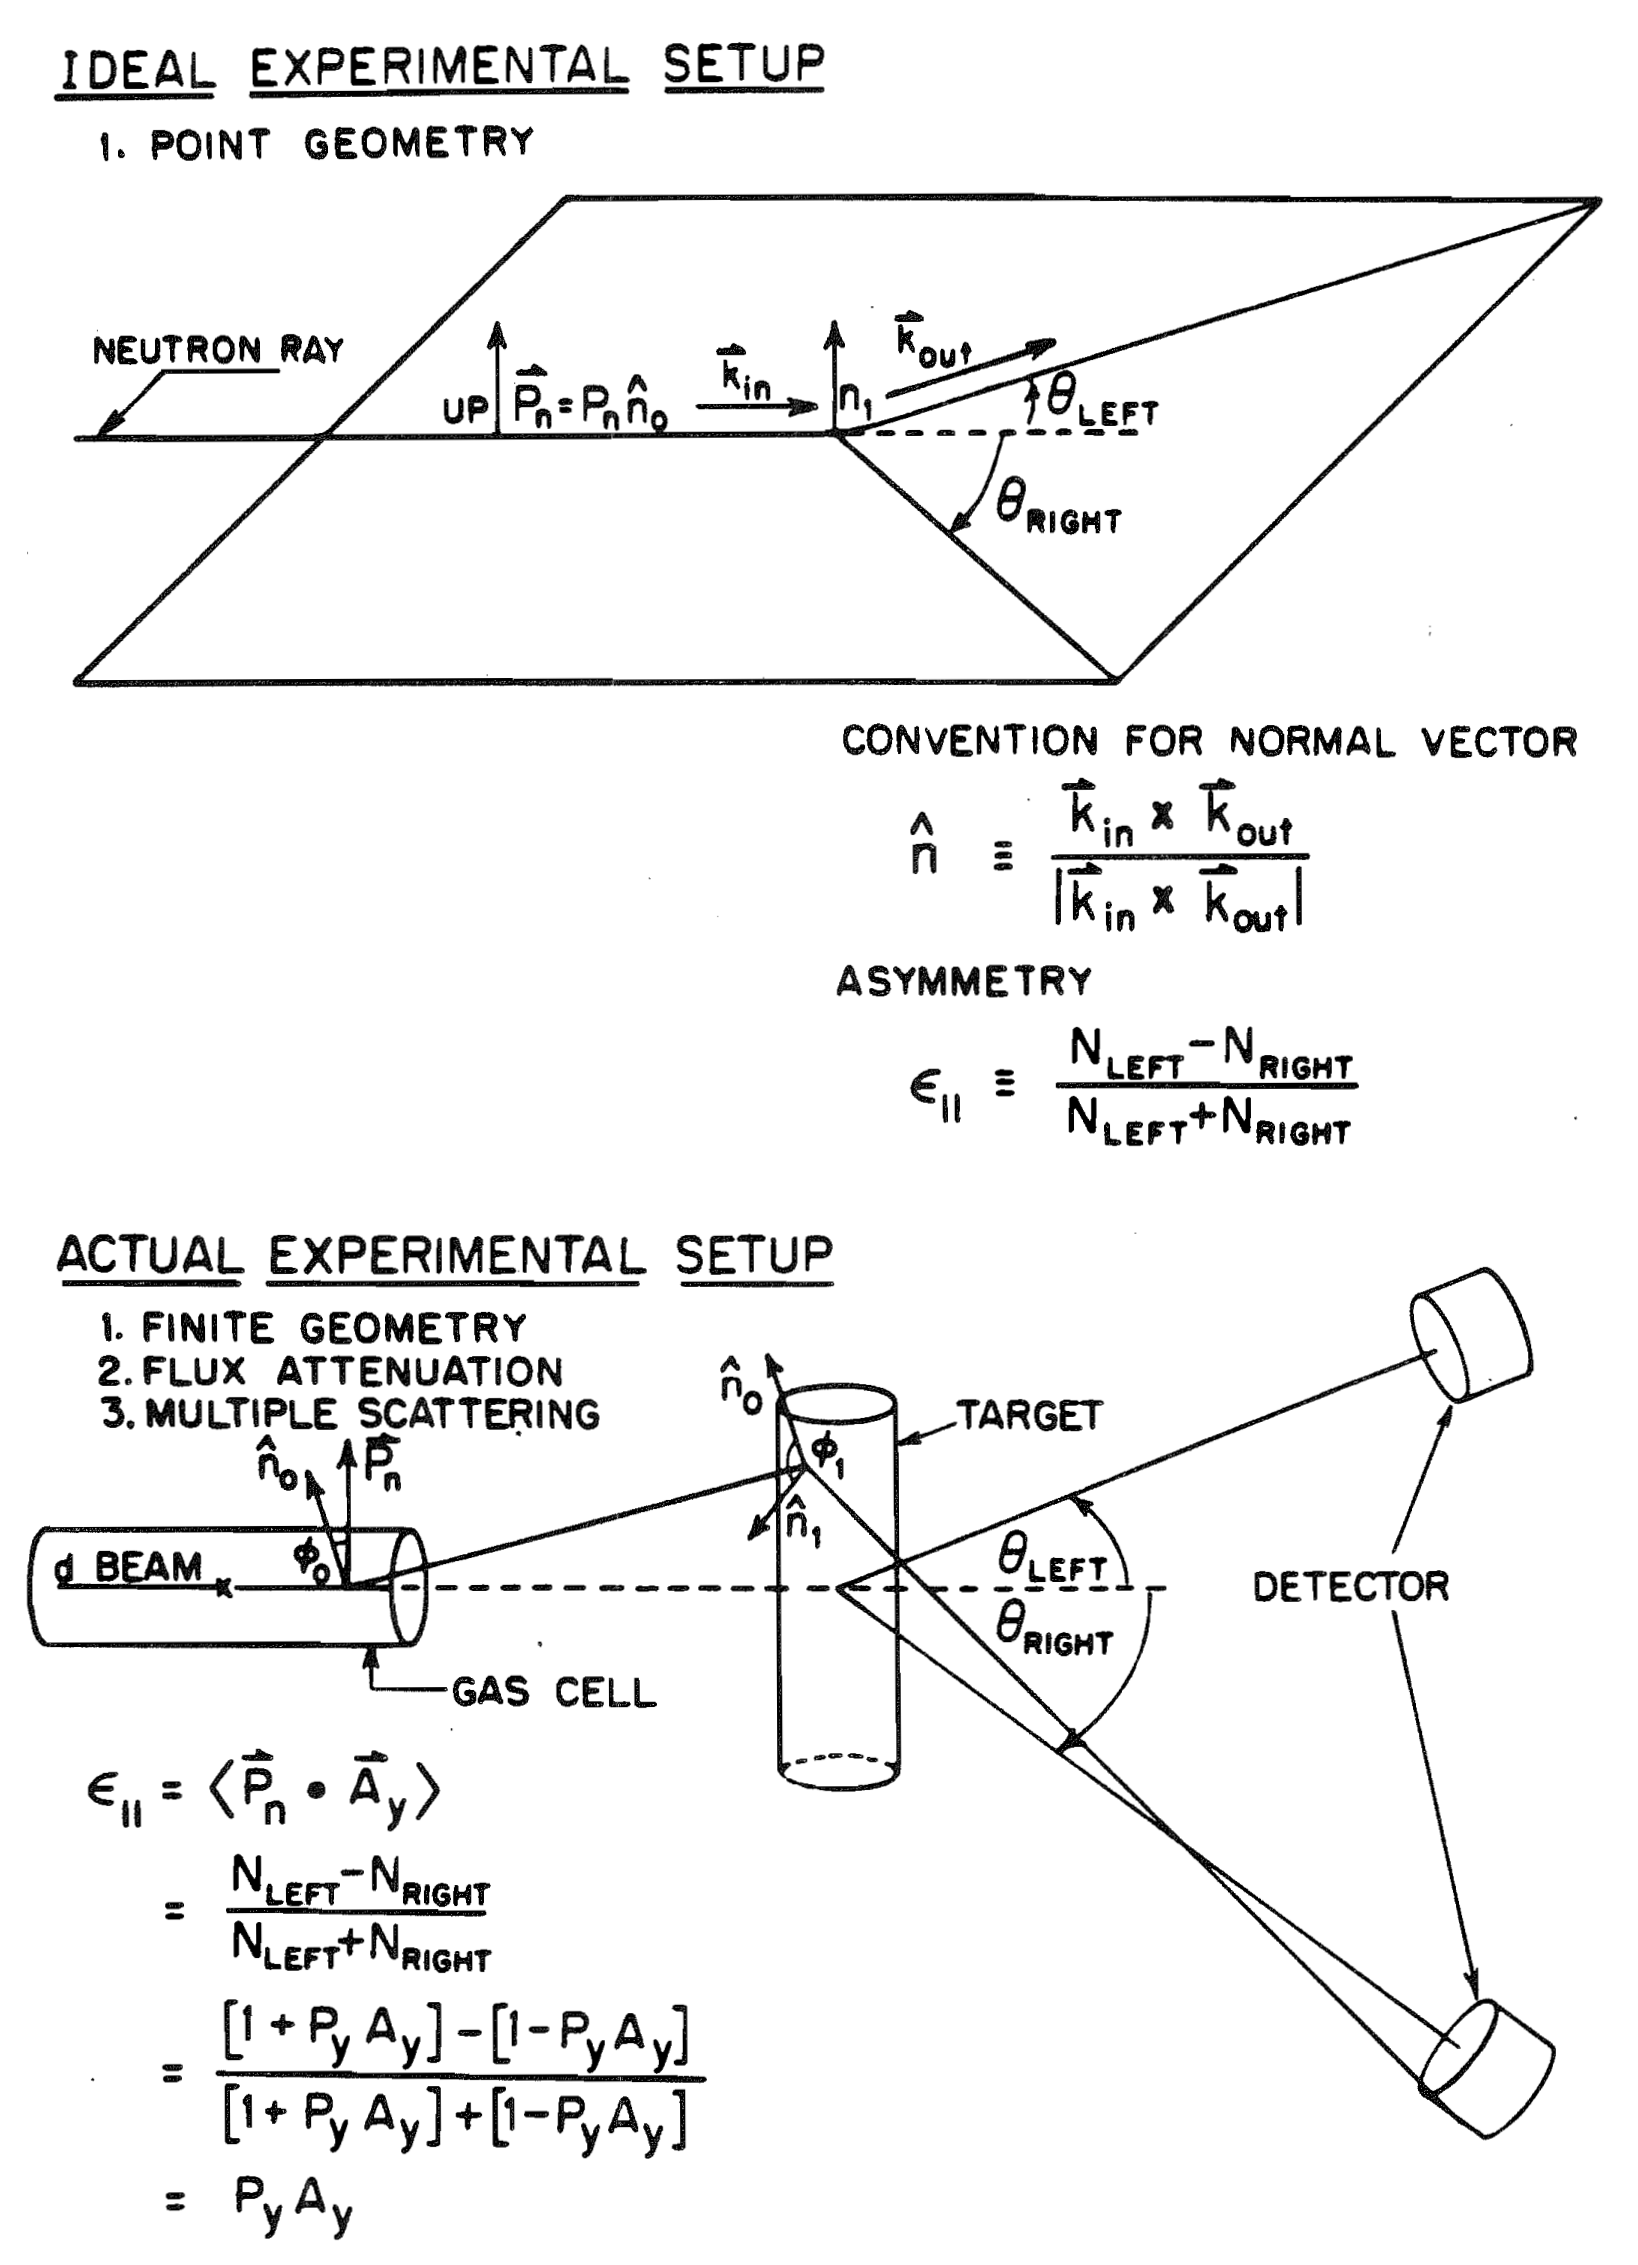
\includegraphics[height=0.7\textheight]{figures/GussFiniteSizeDiagram.png}
        \caption[Illustration of finite-size effects relevant for \el\ cross
        section measurements]
        {
            Illustration of finite-size effects relevant for \el\ cross
            section measurements, from the PhD thesis of P. Guss
            \cite{GussPhDThesis}. Due to the uncertainty in the exact path taken
            by neutrons during scattering and the possibility of multiple
            scattering in the sample, a series of finite-size corrections
            must be applied to recover the true cross section.
        }
        \label{GussFiniteSizeDiagram}
\end{figure}
The experimenter is responsible
for applying appropriate corrections to make results size- and
apparatus-independent. The finite-size analysis for
a similar TUNL-based neutron \el\ measurement on $^{116,120}$Sn is described in detail
in \cite{GussPhDThesis}. In their analysis, Monte Carlo simulations using the
EFFIGY code were
prepared to generate a correction for geometric uncertainty of the neutron
scattering track, the possibility of multiple scattering
in the samples, and flux attenuation in the sample.
For the isotopic Ni and Sn samples they studied, they generated finite-size
corrections of roughly 1-10\% depending on the scattering angle. As seen in
Fig. \ref{GussFiniteSizeEffect}, the
biggest effect is on the depth of the diffraction minima.
\begin{figure}[tb]
    \centering
    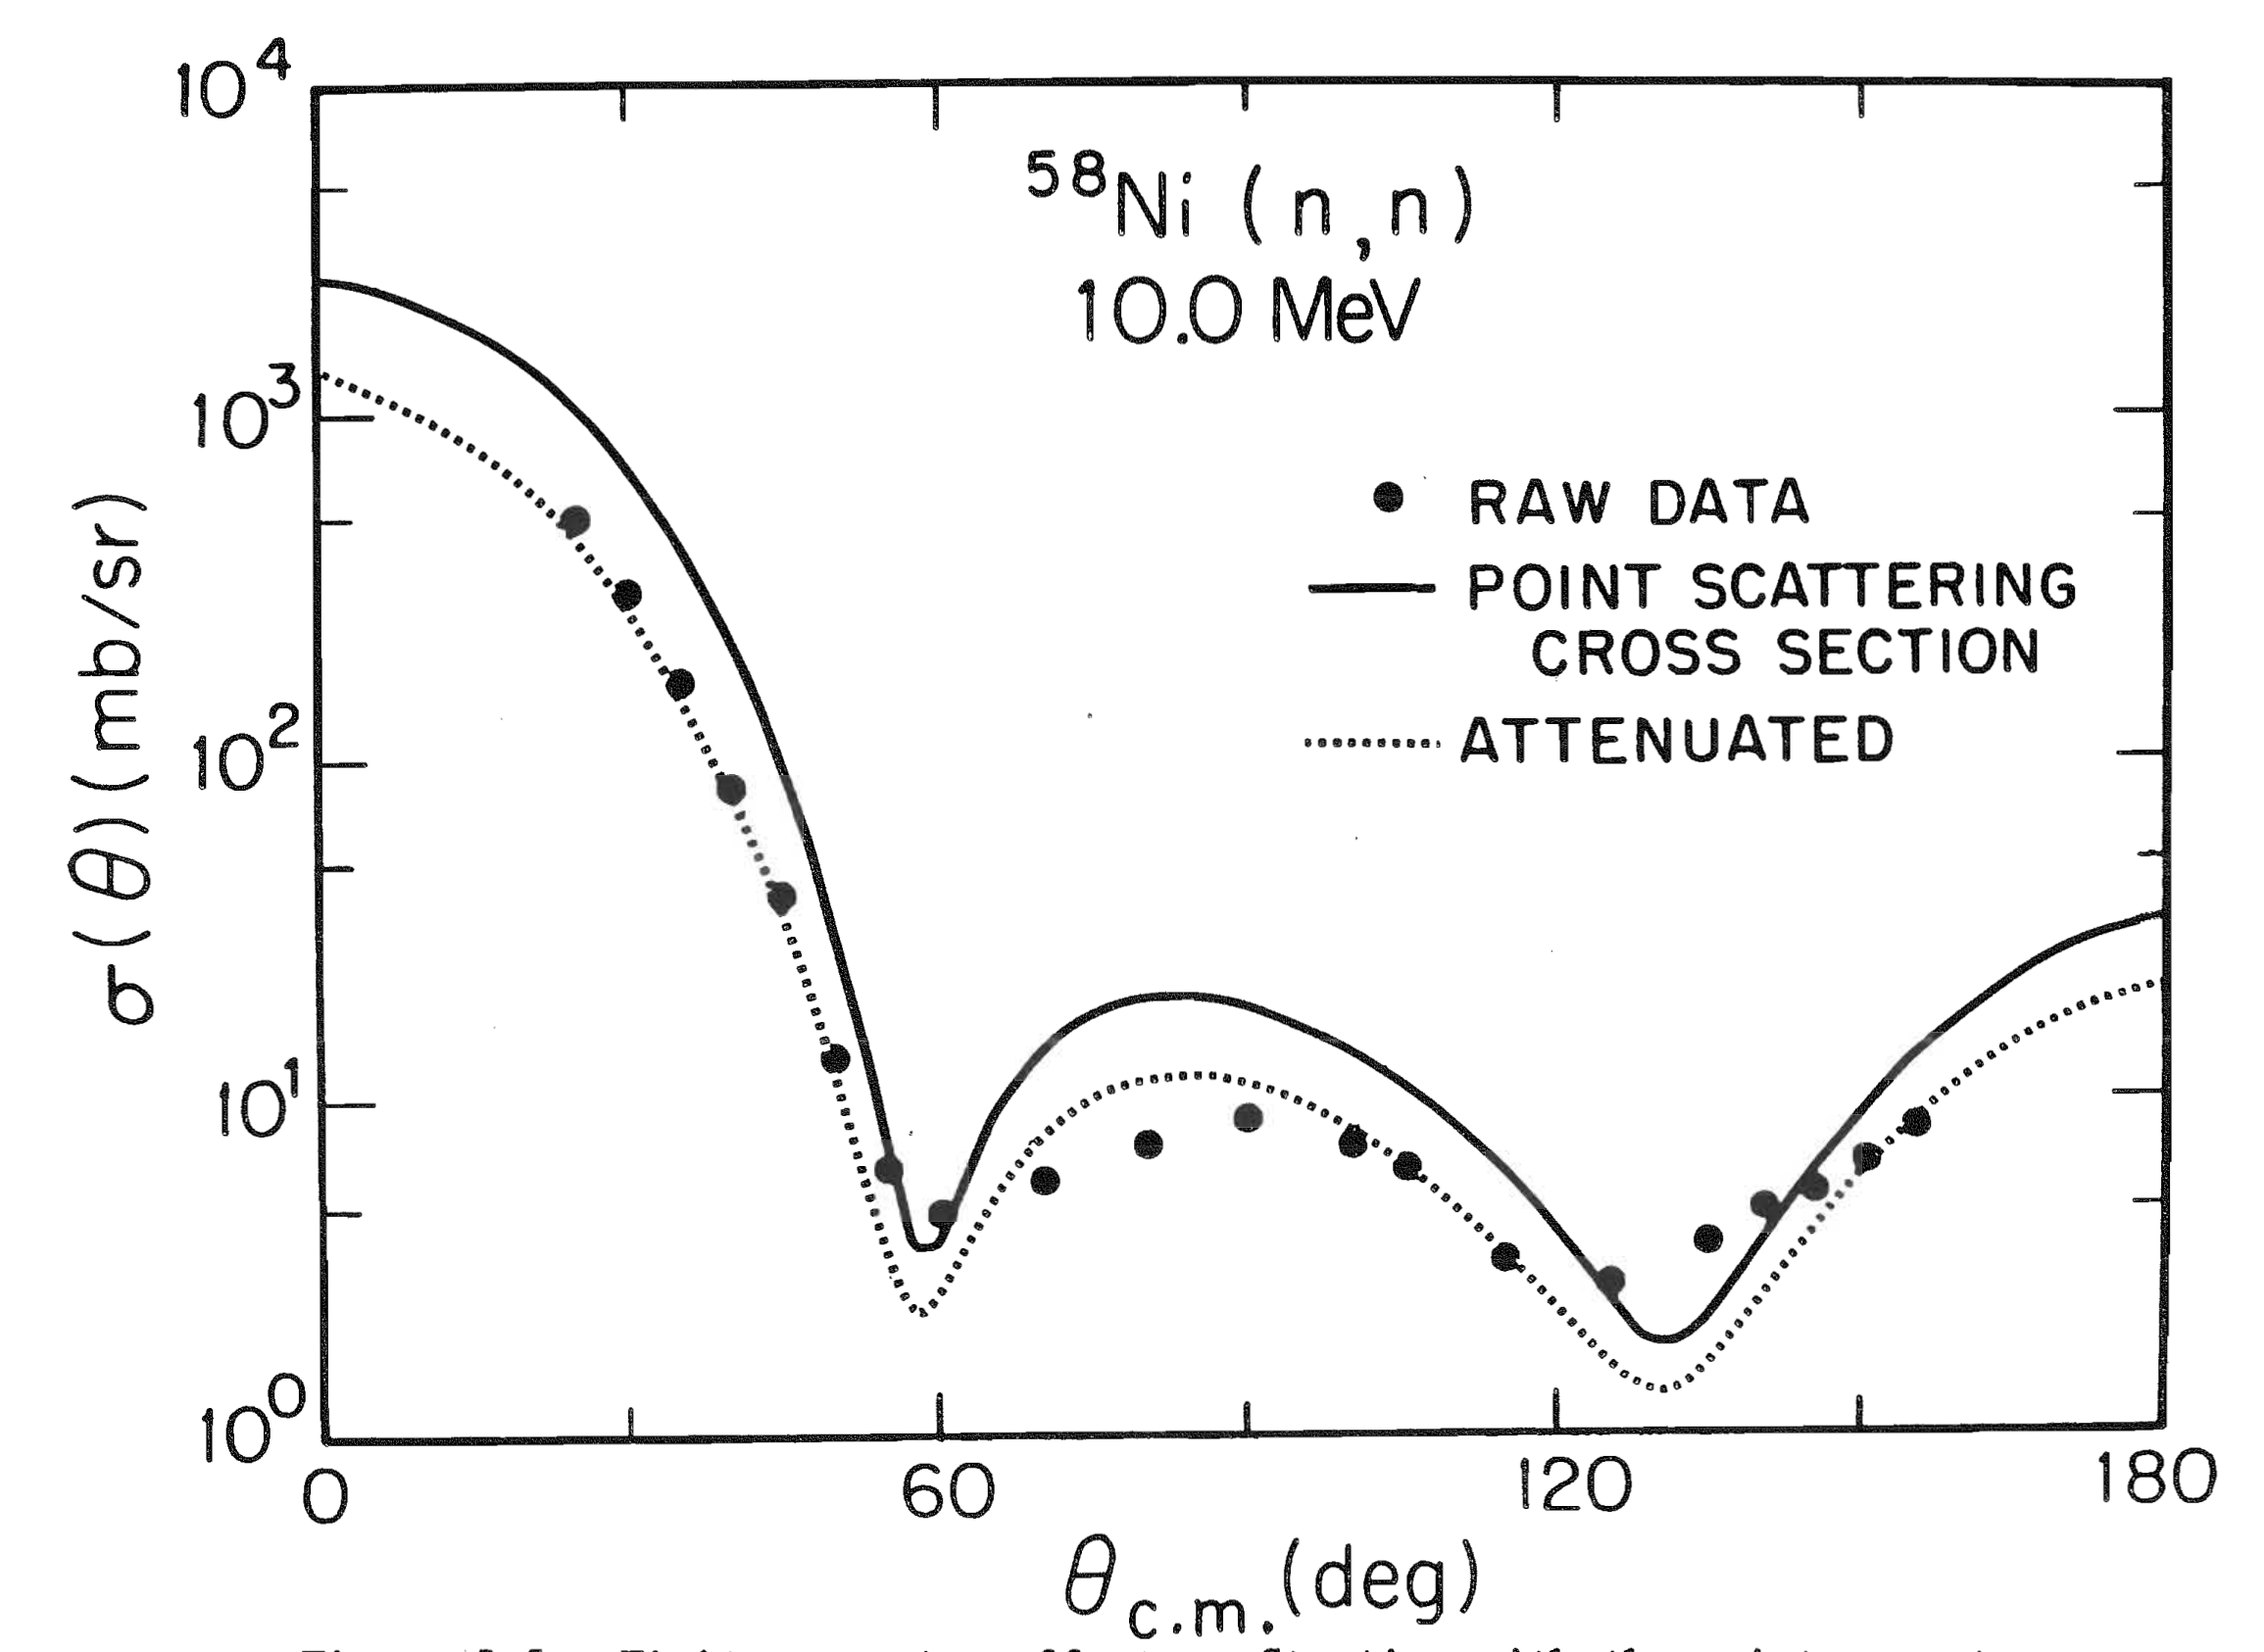
\includegraphics[width=0.9\textwidth, trim={0 0.1cm 0 0}, clip]{figures/GussFiniteSizeEffect.png}
    \caption[Effect of finite-size corrections on previous TUNL neutron \el\ measurement]
    {
        The extent of \gls{finite-size corrections} on a previous neutron \el\ measurement at
        TUNL are shown. Figure is from the PhD thesis of P. Guss \cite{GussPhDThesis}.
        The raw data from this measurement on Ni isotopes are shown as data
        points. Using a Monte Carlo simulation, the authors of the previous
        study generated a correction accounting for multiple scattering in
        their samples, the angular uncertainty stemming from the volume
        of their samples, resulting in the dashed curve. With beam
        attenuation also considered, the cross section is uniformly
        increased across the angular range, giving the solid curve, which
        they take to be the ``true'' cross section. Because our targets are
        approximately an order of magnitude smaller, we see smaller
        finite-size effects in our simulation (see Figs.
        \ref{finiteSizeCorrections} and \ref{multipleScattering}).
    }
    \label{GussFiniteSizeEffect}
\end{figure}
\begin{figure}[tb]
    \centering
    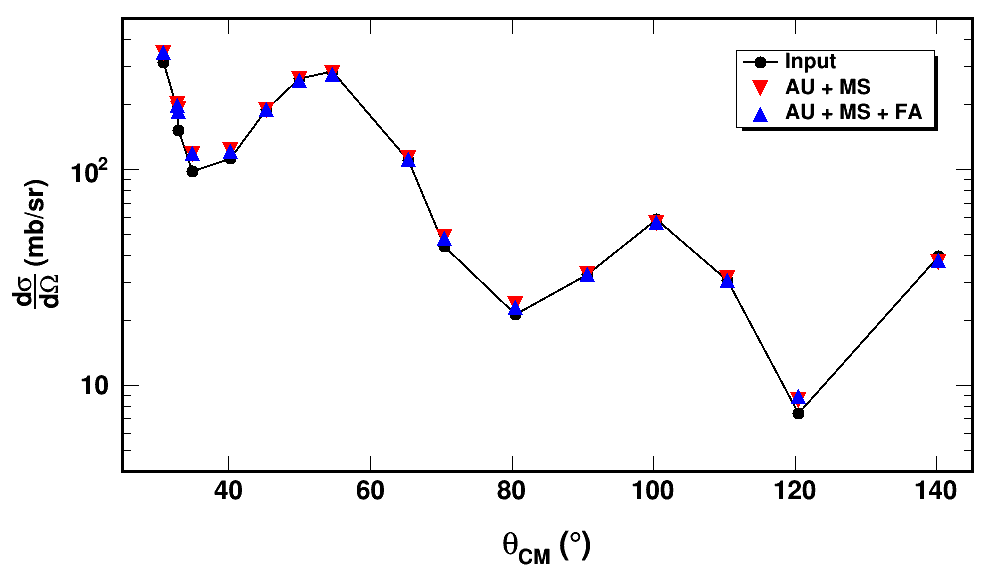
\includegraphics[width=0.9\textwidth]{figures/finiteSizeCorrections.png}
    \caption[Effect of finite-size corrections on our neutron \el\ measurement]
    {
        The extent of our finite-size corrections are shown, per the output
        of a typical finite-size simulation. Our raw 11 \mega\electronvolt\ \snFour \el\ data
        are shown as black points (connected with lines to guide the eye) and
        were used as the input cross section for the finite-size simulation.
        The simulation scattered neutrons according to the input distribution
        that were scored on an array of detectors with the same geometry
        as in the experiment. ``Output'' cross sections were calculated based on
        the number of detector hits. The results of two simulations are shown:
        one including only the effects of
        angular uncertainty (AU) and multiple scattering (MS), shown by red
        triangles, and the other also included flux attenuation in the target
        (FA), shown as blue triangles. For our targets, the finite-size effects
        were an order of magnitude smaller than those of
        \ref{GussFiniteSizeEffect}, as anticipated given the size of our targets.
    }
    \label{finiteSizeCorrections}
\end{figure}
However, their samples
were an order of magnitude larger than our
samples: 42.59 g and 44.73 g for their \snSixteen\ and \snTwenty\ samples,
respectively, compared to 4.97 g and 5.55 g for our \snTwelve\ and \snFour\
samples. Thus we anticipated a significantly smaller correction would be
required.
\begin{figure}[tb]
    \centering
    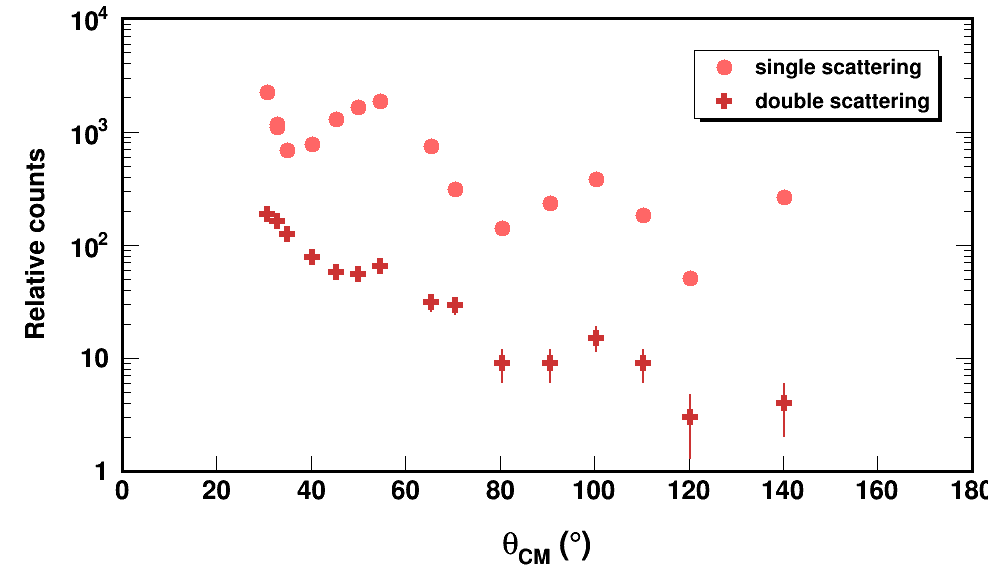
\includegraphics[height=0.4\textheight]{figures/multipleScattering.png}
    \caption[Relative counts due to multiple scattering in the sample volume]
    {
        Relative counts due to single scattering and double scattering
        in the sample volume, per our finite-size simulation on \snFour. The
        measured data from our experiment include scattering to all orders. Our 
        simulation shows that the contribution from double scattering (and
        higher orders) is quite small and makes an appreciable difference only
        in the depth of the diffraction minima.
    }
    \label{multipleScattering}
\end{figure}
Figure \ref{GussFiniteSizeDiagram} illustrates the potential for multiple scattering in the samples
and the small degree of angular uncertainty in the neutron scattering path.
The effect of this angular uncertainty on the measured cross
sections is to ``wash out'' the sharp diffraction minima expected to be present in the true cross
section. To assess the magnitude of this effect from our
samples, an iterative simulation was prepared in which a uniform beam of neutrons
impinged on the sample volume and was scattered into the time-of-flight
detectors. To select each neutron's scattering path, we took the
raw cross section from our measurement to be the true cross section and allowed
neutrons to propagate through the sample and scatter up to twice. After
scattering, neutrons were scored in simulated detectors with the same dimensions
used in the real experiment and an ``output'' cross section was generated. The
output is thus a weighted convolution of the input cross section
over the finite-size effects of the samples and detectors. In addition to
running a simulation with the sample sizes used in the experiment, we performed
addition simulations with exaggerated sizes for the
sample to make finite-size effects more visible. A comparison between the input
and output cross sections shows the effects of beam attenuation and angular
uncertainty, seen in Figs. \ref{finiteSizeCorrections} and
\ref{multipleScattering}.
To calculate correction factors, we divided the simulation's
input cross section by the output cross section for each angle and multiplied our
experimental results by this factor. In principle, this procedure to generate
the correction should be repeated iteratively, with the new corrected cross
section plugged back into the simulation, but in practice the corrections for
our data were so small that only the first iteration was required.
\section{Results}
\subsection{\snTwelveFour\ \el\ at 11 \mega\electronvolt}
Figure \ref{SnECS_11MeV} shows our final results for \snTwelveFour\
\el\ at 11 \mega\electronvolt\ after applying the corrections above. Our data on \snFour\
at 11 \mega\electronvolt\ are in reasonable agreement with those of Rapaport et al.
\cite{Rapaport1980}, which were taken using a much larger enriched sample
($\approx\frac{1}{3}$ mol) at the University of Ohio neutron time-of-flight
facility. At angles just less than diffraction minima (e.g., at
angles of 65-70\textdegree), the \snTwelve\ \el\ is seen to be larger
than that of \snFour, a consequence of nuclear size
differences leading to a phase mismatch, similar to the effect in the \oSixEight\
\tot\ relative difference of Fig. \ref{IsotopicDifferenceO}. This same
phase-mismatch trend is
visible in the $^{116,118,120,122,124}$Sn \el\ collected by Rapaport et al.,
though the effect is less dramatic as the isotopic range is smaller.
Due to our small \snTwelveFour\ sample sizes,
our statistics in the 80\textdegree\ and 120\textdegree\ diffraction minima are
limited, leading to a large uncertainty in the \el\ relative difference between
\snTwelveFour.

\begin{figure}[tb]
    \centering
    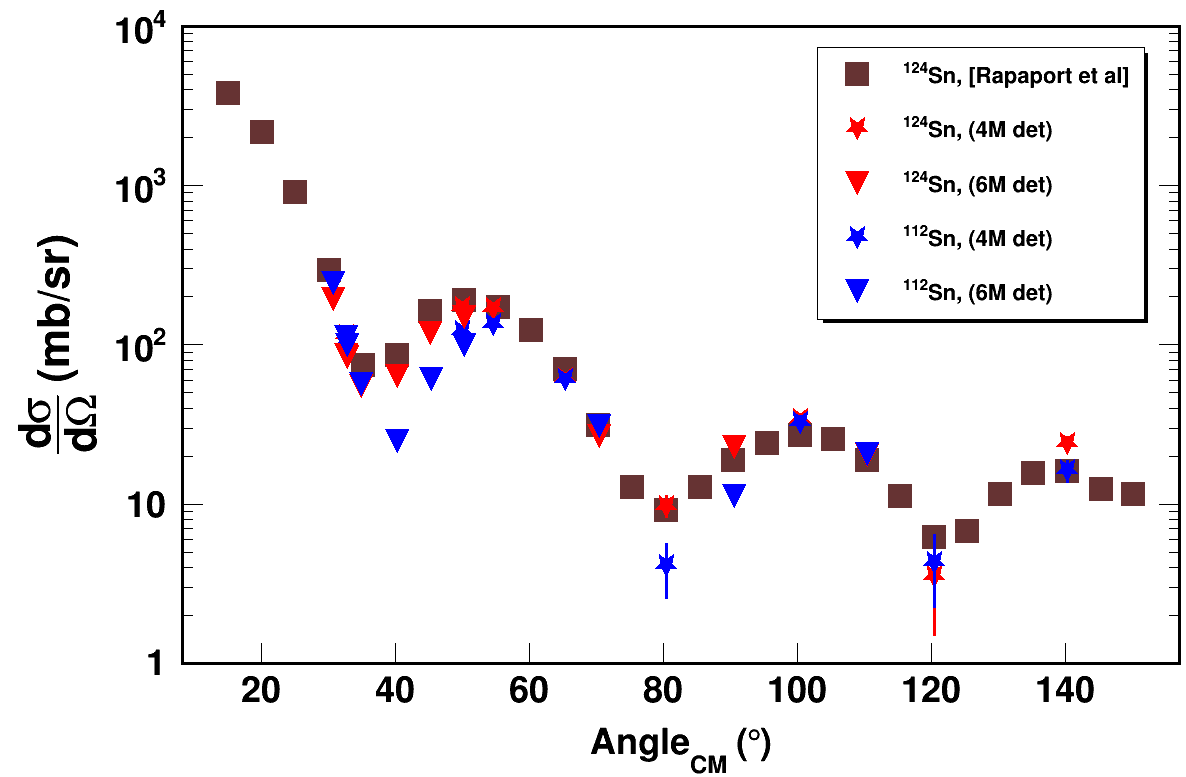
\includegraphics[width = 1.0\textwidth]{figures/ECSResults2017.png}
    \caption[Neutron \el\ on \snTwelveFour\ at 11 \mega\electronvolt: our results and literature data]
    {
        Neutron \el\ on \snTwelveFour\ at 11 \mega\electronvolt: our results and data on
        \snFour\ from Rapaport et al. \cite{Rapaport1980}. The data collected
        with the 4M detector are shown as stars, and the data collected
        with the 6M detector are shown as triangles. At 32.5\textdegree and
        50\textdegree, data were taken with both 4M and 6M detectors at separate
        times, and results from the two independent detectors are in reasonable agreement.
    }
    \label{SnECS_11MeV}
\end{figure}

\subsection{\snTwelveFour\ \el\ at 17 \mega\electronvolt}
Figure \ref{SnECS_17MeV} shows our final results for \snTwelveFour\
\el\ at 17 \mega\electronvolt\ after applying the corrections described above. Our data on \snFour\
at 17 \mega\electronvolt\ are in reasonable agreement with those on \snTwenty\ of Guss et al.
\cite{Guss1989, GussPhDThesis}, which were taken at the same TUNL neutron
time-of-flight facility using an enriched sample roughly ten
times larger than ours. The same phase-mismatch effect is visible to the left of
the diffraction minima (e.g., at 70\textdegree). Above 100\textdegree, we were unable
to collect sufficient statistics to recover a precise \snTwelveFour\ \el\
relative difference, a consequence of the reduced cross section at 17 \mega\electronvolt\
compared to 11 \mega\electronvolt. Whereas in the 11 \mega\electronvolt\ dataset, the 4M and 6M detectors were in
good agreement, in the 17 \mega\electronvolt\ dataset, our results from the 4M detector appear
to be systematically slightly lower than those from the 6M detector, likely due to the
increased difficulty in resolving the elastic from the inelastic scattering
peaks in the 4M detector at 17 \mega\electronvolt, especially at low angles. As with the \tot\
results presented in Chapter \ref{TCSAnalysis}, the relative difference between
isotopes (relevant for fixing the isovector strength) should be insensitive to any systematic 
errors in our measurement.

As with the 11 \mega\electronvolt\ dataset, the biggest difference between the
\snTwelveFour\ \el\ data is at the first diffraction minimum from
30-40\textdegree. The cross section in this low-angle region is expected
to be sensitive to the interaction of the incident neutron
with the nuclear surface rather than with the nuclear core, which
is better probed with backward-angle scattering. Connecting the shape and
magnitude of these \el\ results with the shape and magnitude of the nuclear
potential is the subject of Chapter \ref{DOMResults}.

\begin{figure}[tb]
    \centering
    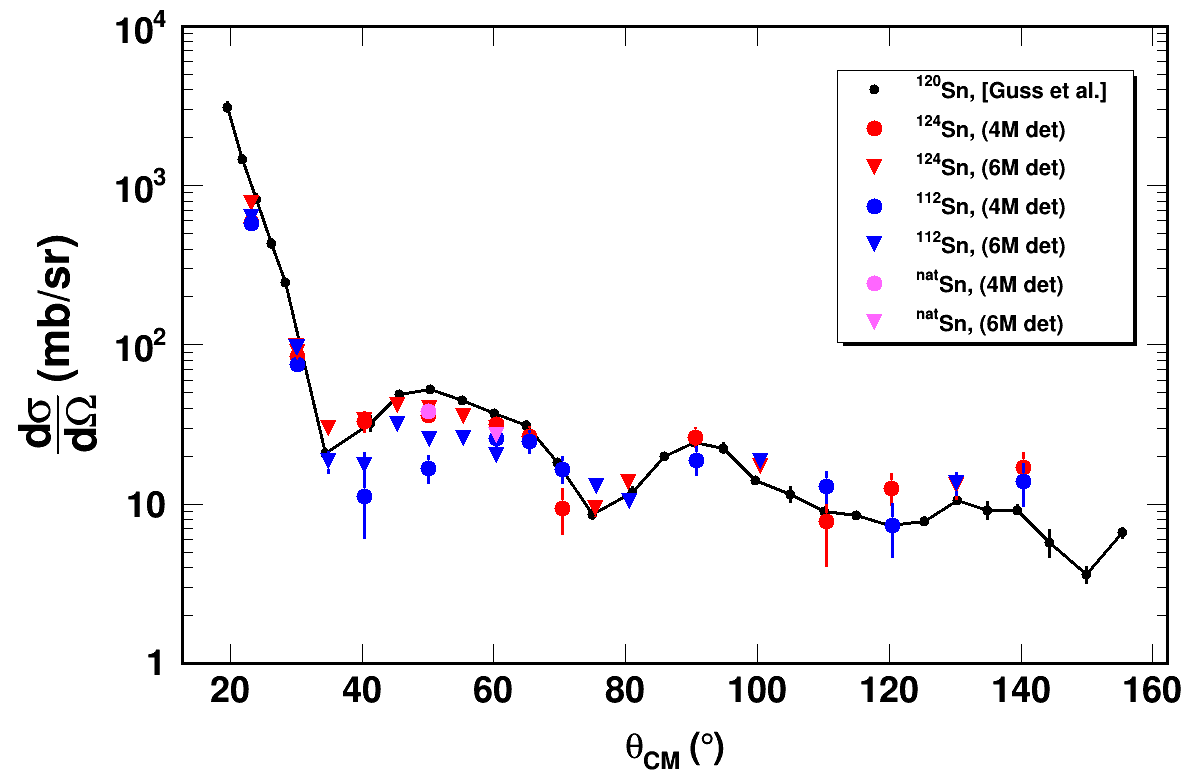
\includegraphics[width = 0.9\textwidth]{figures/ECSResults2018.png}
    \caption[Neutron \el\ on \snTwelveFour\ at 17 \mega\electronvolt: our results and
    literature data]
    {
        Neutron \el\ cross sections on \snTwelveFour\ at 17
        \mega\electronvolt: our results and data on \snTwenty\ from Guss et al.
        \cite{Guss1989}. The data collected with the 4M detector
        are shown as stars, and the data collected
        with the 6M detector are shown as triangles. In addition to data on
        \snTwelveFour, we collected data on \snNat\ at 50\textdegree\ and
        60\textdegree, shown in pink. The data on \snNat\ lie halfway between our data on
        \snTwelve\ and \snFour, adding confidence that the relative difference
        between \snTwelveFour\ is accurate. At 30\textdegree,
        40\textdegree, and 50\textdegree, data were taken with both 4M
        and 6M detectors at separate times, and results from the two independent
        detectors are in rough agreement, though results from the 4M detector appear
        to be systematically slightly lower at low angles.
    }
    \label{SnECS_17MeV}
\end{figure}

\afterpage{\clearpage}
